%!TEX root = ../document.tex
\chapter{基于自注意力机制的序列感知推荐}

\section{问题的提出}
在多个不同的机器学习领域,例如图像描述、机器翻译、阅读理解、摘要生成还有一些其他的应用上,已经证明注意力机制是有明显效果的%
这一机制背后的重要思想是影响序列输出的因素只与序列中某些重要信息相关,而无需过多关注其他无用的信息。这一机制的命名受到人类视觉系统中视觉焦点的启示,所以称为注意力机制。

2017年NIPS大会上谷歌发表了一个完全用注意力机制构建的机器翻译框架\textit{Transfomer}\upcite{NIPS2017_7181},到达了当时最好的效果。


在基于循环神经网络的序列感知推荐系统方面,由于循环神经网络本身的特性也带来了性能上面的一些缺陷。由于循环神经网络的结构,当前神经元的输入有上一个神经元的输出,反向传播梯度更新时,下一个神经元的梯度更新也需要上一个神经元计算完再开始,这一串行的性质限制了循环神经网络的训练速度,特别是当需要使用更深的循环神经网络的时候。而由于自注意力机制完全抛弃了循环神经网络的串行结构而依然能捕获数据的序列关系,近来已成为序列建模领域的研究热点。
使用注意力机制的另一好处是基于注意力的方法在推荐可解释性方面也更好说明。%
因此在这一部分,我们为了进一步的提升基于双向循环神经网络的序列感知推荐算法,本章基于编码器解码器框架,选用自注意力机制作为编码器和解码器的特征提取器,来建模用户短期行为模式的依赖因素。

其整体框架结构如图\ref{fig:transformer}所示。

\begin{figure}[htb]
  \centering
  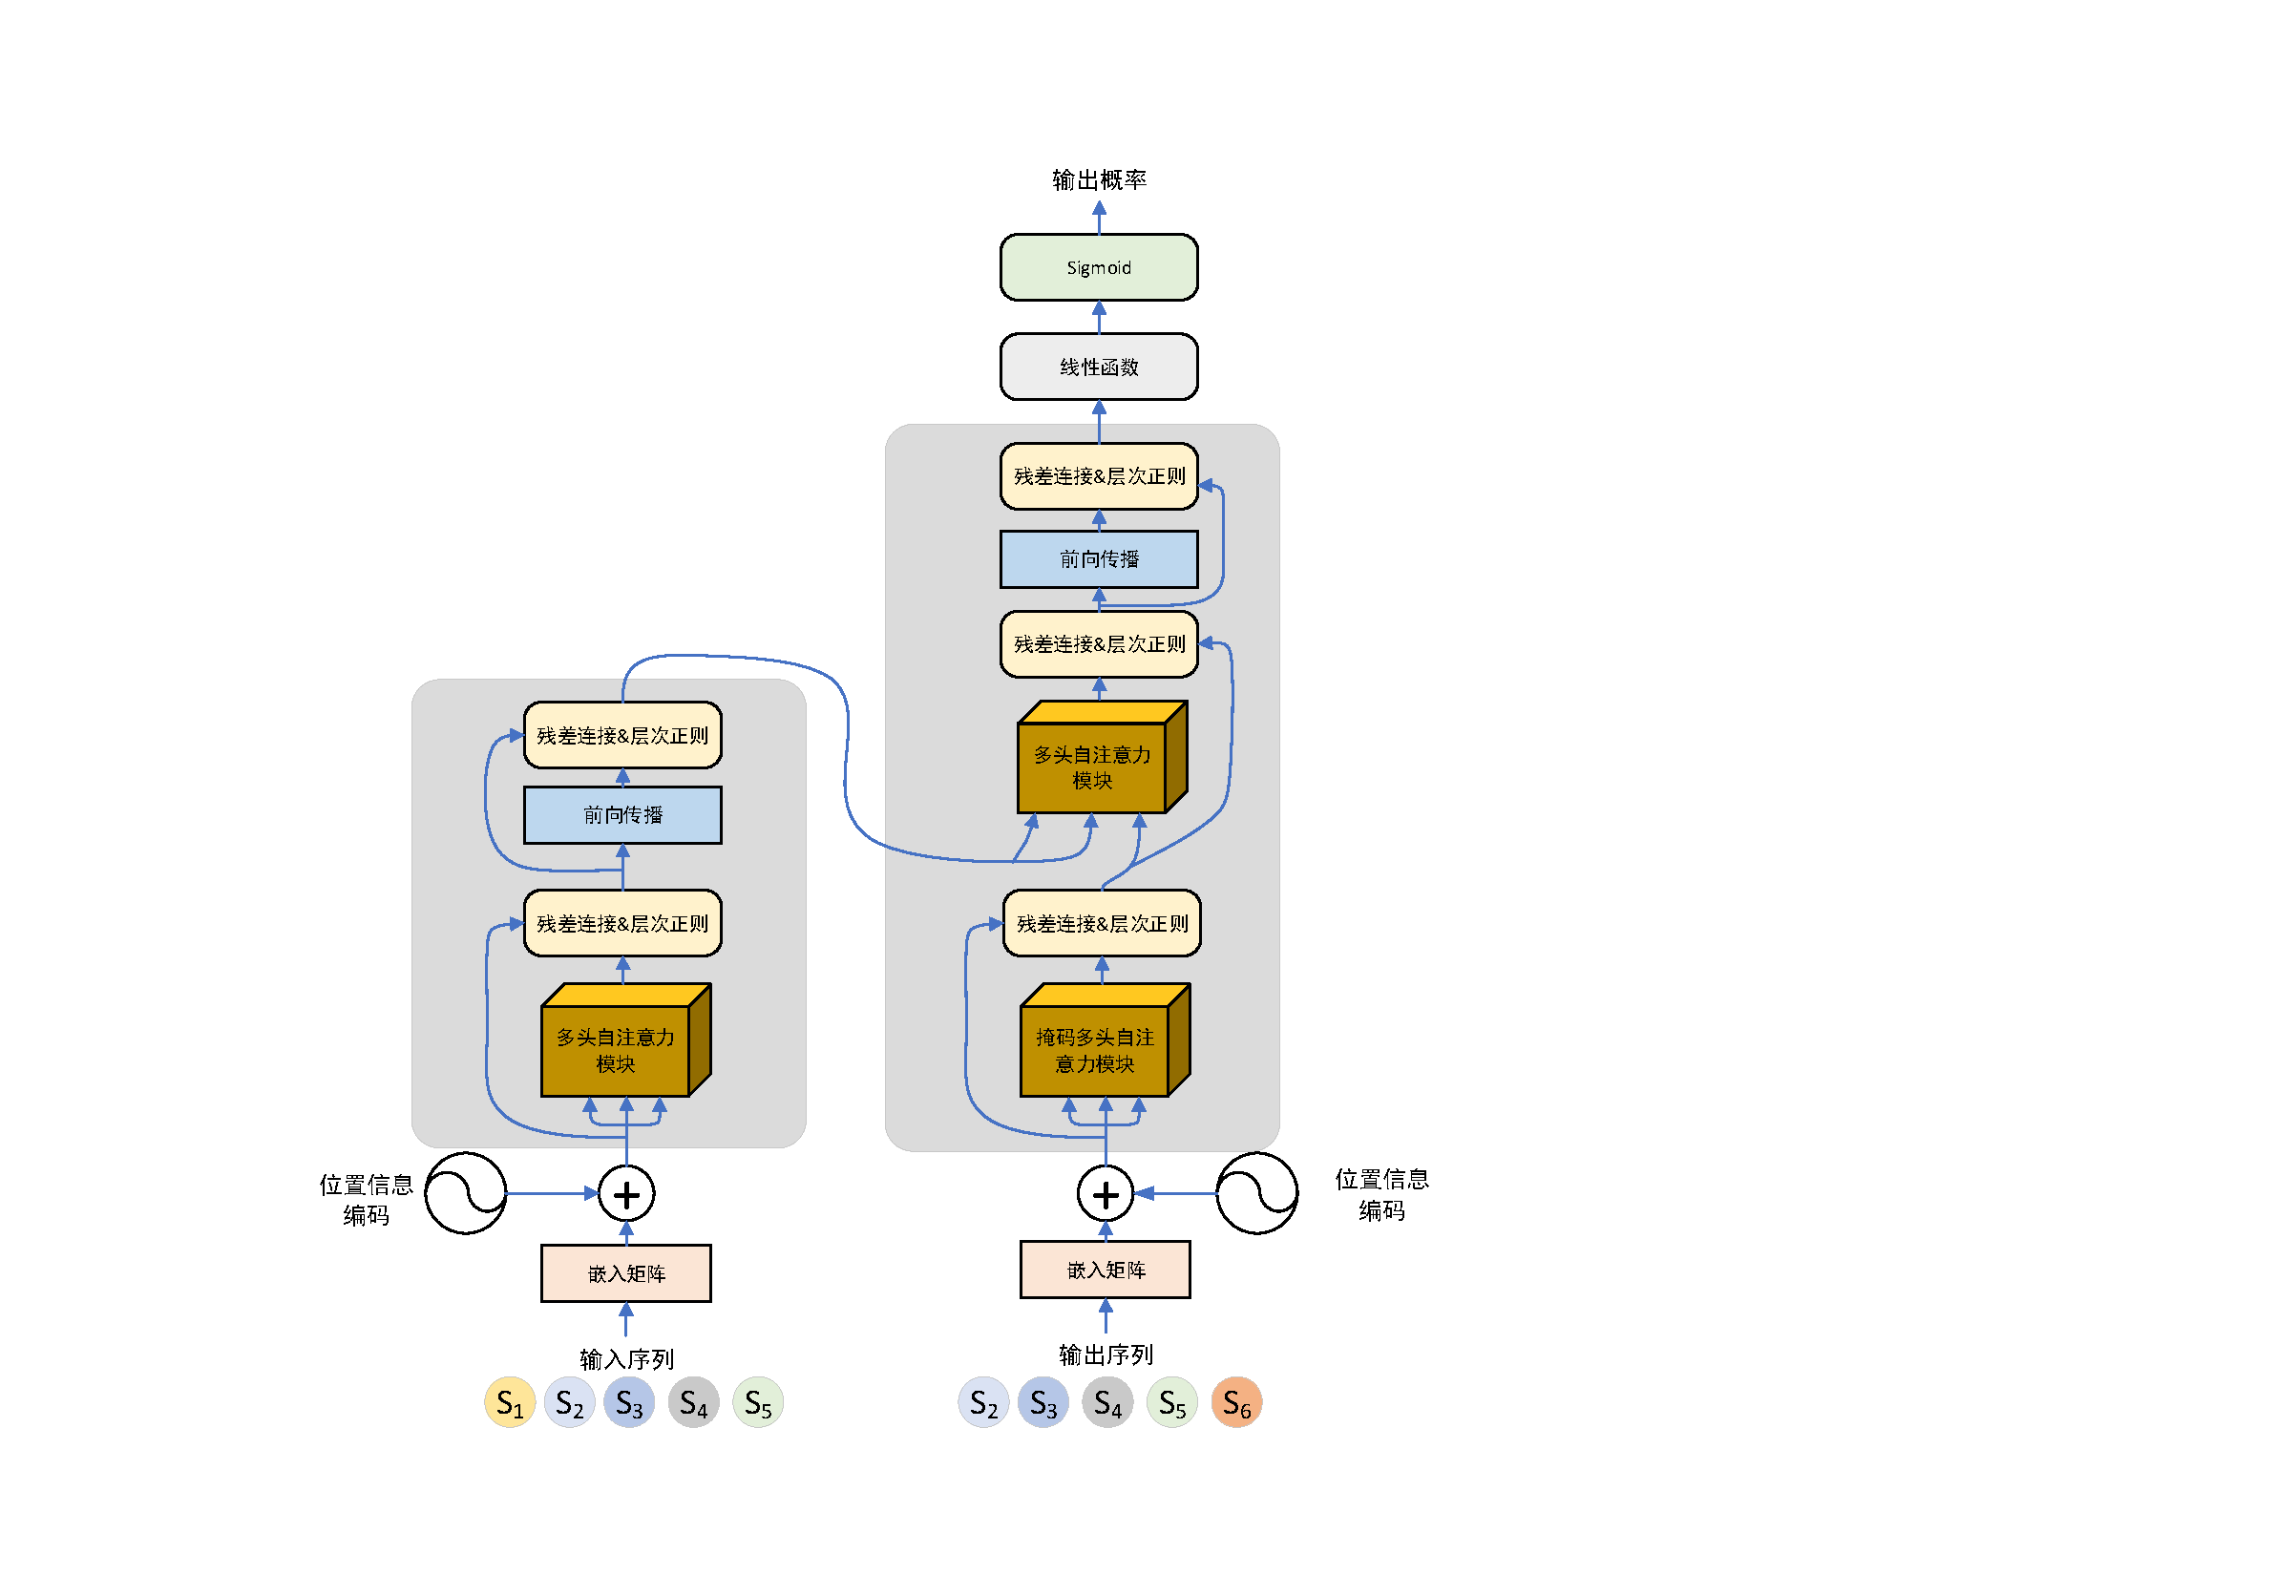
\includegraphics[width=\linewidth]{transformer.pdf}\\
  \caption{基于自注意力机制的序列推荐算法框架图}
  \label{fig:transformer}
\end{figure}

\subsection{目标问题定义}

与第三章中基于双向长短期记忆网络的序列感知推荐模型问题一样,我们定义$\mathbb{U}= \left \{ u_{1},u_{2},...,u_{N} \right \}\label{eq}$%
代表不同的用户集合,定义$\mathbb{I}= \left \{ i_{1},i_{2},...,i_{M} \right \}$代表在所有序列%
中出现过的不同物品集合,$s_{u}^{t}\in \mathbb{I}$表示用户$u$在时间刻$t$点击某一个物品的记录,%
该记录对应的物品包含在物品集合$\mathbb{I}$当中。对于每一个用户$u$,%
都记录一个按照数据诞生时间戳顺序排列的用户点击记录%
序列$\mathbb{S}_{u}=\left \{ s_{u}^{1},s_{u}^{2},...,s_{u}^{t-1},s_{u}^{t} \right \}$%
序列感知推荐的目标是预测下一次点击行为,也就是做出$t+1$时刻的推荐$s_{u}^{t+1}$。在序列感知推荐%
模型当中,对于序列$s$,模型的输出是所有候选物品对象可能被点击的概率$\hat{y}$,而概率最大的$K$个%
输出所对应的候选物品将作为推荐项目给到用户。%

\subsection{嵌入层}

序列中的物品ID不具有实际数学意义,因此不能把ID编码直接%
传输给计算机进行计算,但为了使计算机能够以较少的资源消耗而感知不同的物品身份,这里同样不使用One\_hot编码%
而使用与基于双向长短期记忆网络的序列感知算法一样的嵌入矩阵\upcite{Mikolov:2013:DRW:2999792.2999959}来对物品ID进行处理:
$$
e(I_i) = EI_i
$$
其中$E\in \mathbb{R}^{|e|\times |M|}$, $|e|$是嵌入层的大小,$|M|$是训练集中不同项目的数量。%
所以$e(I_i)$是$I_i$的嵌入表达,其是一个具有$e$个实数的稠密矩阵。

\textbf{位置信息嵌入层}

由于在利用自注意力方法构建的模型当中,没有了循环和卷积结构,因此抛弃了项目之间的序列信息,但%
用户的短期兴趣关注点隐藏在序列之中,为了使我们的模型能够捕捉到序列变化信息,必须将序列中物品%
的相对或者绝对位置信息加入到模型当中去。位置编码有可学习形式(learned)和固定参数形式%
(fixed)\upcite{DBLP:journals/corr/GehringAGYD17}。这里我们使用了与%
\textit{Transfomer}\upcite{NIPS2017_7181}一样的方式,在模型输入的嵌入层中加入物品序列的固定参数形式“位置编码”,%
即位置信息嵌入层。我们使用正弦和余弦函数并结合不同频率将物品的固定位置编码传递给模型,位置编码%
的一个维度对应于正弦曲线上的一个值,从而形成从$2\pi $到$10000 \cdot  2\pi$的几何级数波长,%
这些信号作为额外的信息加入到输入(或输出)中以表达时间的流逝,使模型能够%
感知到当前正在处理的是输入(或输出)序列的哪个部分。:
\begin{align}
  PE(t,2e) &= \sin (t/10000^{2e/d_{model}}) \label{eq:sin}\\
  PE(t,2e+1) &= \cos (t/10000^{2e/d_{model}}) \label{con}
\end{align}
\begin{figure}
\centering
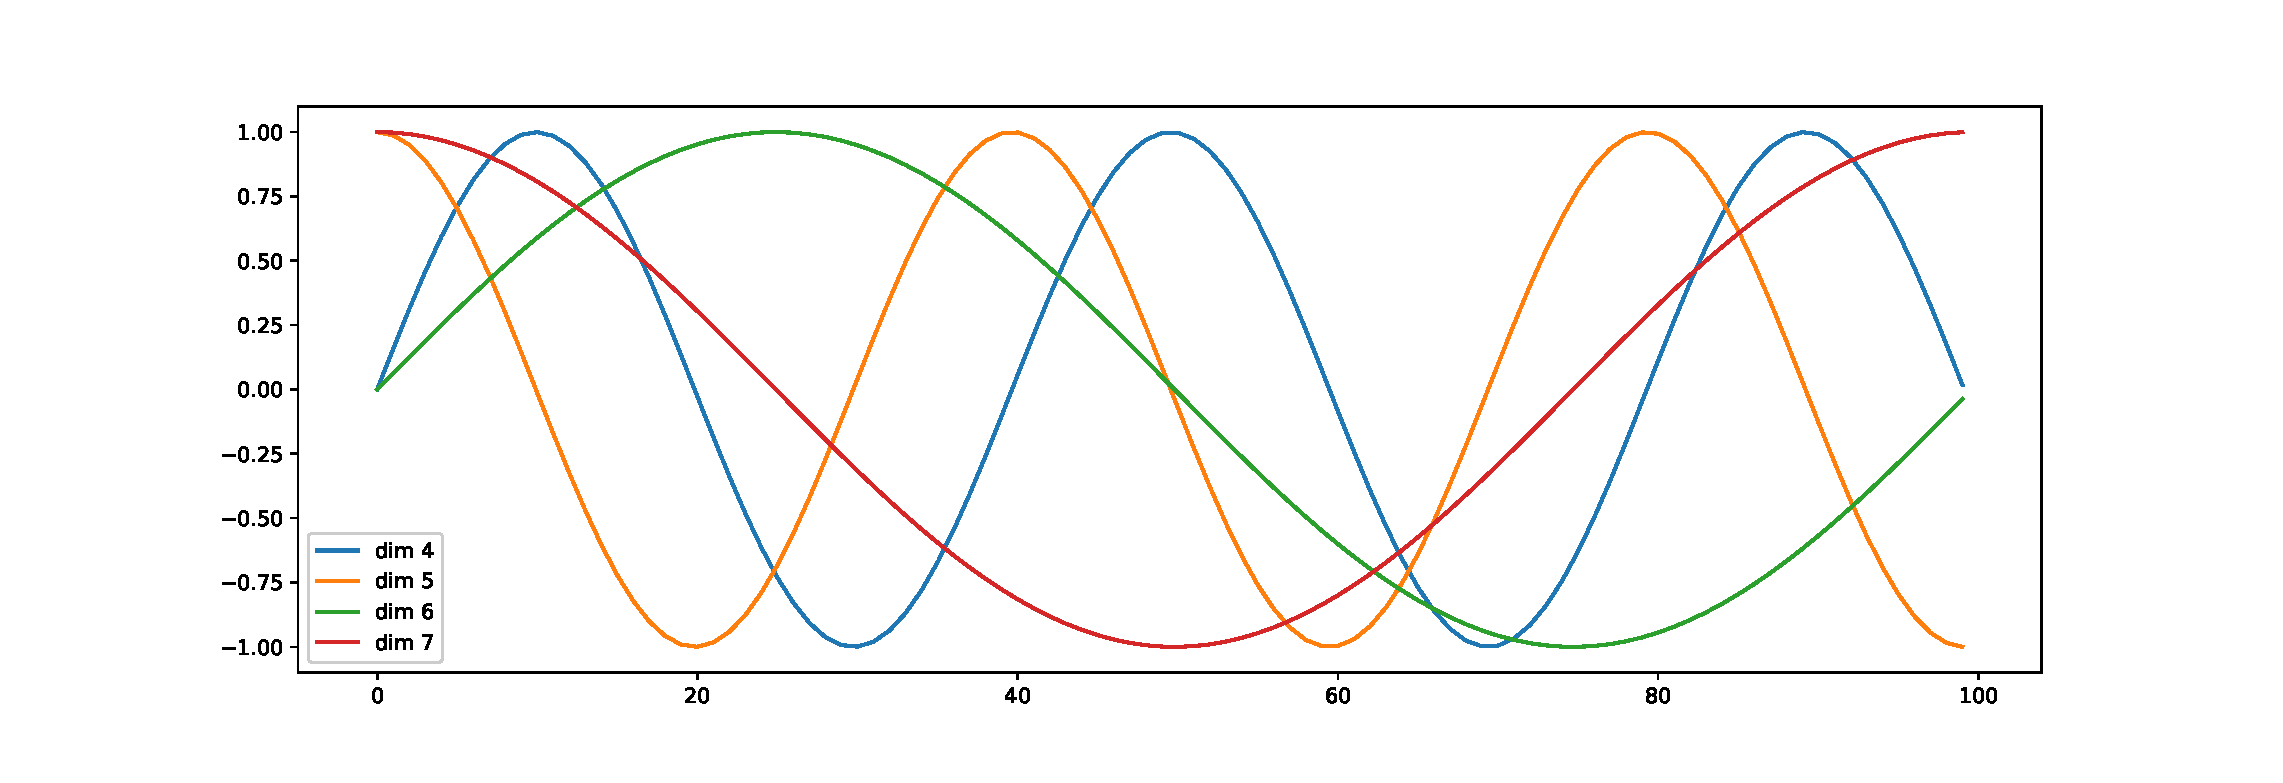
\includegraphics[height=4cm,width=14cm]{pe.eps}
\caption{使用不同维度大小的位置编码波形图}
\label{pe}
\end{figure}

其中$t$就是位置信息,表示该物品出现在序列中的第$t$个时间步骤,$e$是位置嵌入层的维度。图\ref{fig:pe}显示,不同的位置嵌入层维度大小,位置编码波形图具有不同的波长。由于位置信息嵌入层与嵌入层有相同的维度$|e|$,因此可以把两者相加起来构成我们最终的输入嵌入层$\widehat{\mathbf{E}}$:
\begin{equation}
	% \label{equ:chap04:embedding}
	\label{fig:pe}
	\widehat{\mathbf{E}}=\left[ \begin{array}{c}{\mathbf{E}_{s_{1}}+\mathbf{PE}_{1}} \\ 
	{\mathbf{E}_{s_{2}}+\mathbf{PE}_{2}} \\ 
	\cdots \\
	{\mathbf{E}_{s_{n}}+\mathbf{PE}_{n}}\end{array}\right]
\end{equation}

\subsection{编码器解码器框架}
编码器解码器(Encoder-Decoder)框架\upcite{D14-1179,DBLP:journals/corr/GehringAGYD17}是自然语言处理中常用的一种序列生成框架,其常用来构建机器翻译模型。Encoder-Decoder框架由一个解码器(Encoder)和一个编码器(Decoder)构成,
Encoder用来处理输入序列$x_{1},x_{2},x_{3},\cdots ,x_{t-1},x_{t}$,将输入序列处理成语义向量,Decoder用来生成输出序列$y_{1},y_{2},y_{3},\cdots ,y_{t-1},y_{t}$,将处理过的语义向量转换成输出序列。Encoder与Decoder的构建可以根据任务的不同选取具有不同特性的CNN/RNN/BRNN/GRU/LSTM算法。


但在我们的序列推荐框架中,考虑序列中的每一个输入节点,其期望的输出应为其序列中直接后继节点,因此我们可以根据这一性质构建一个Encoder-Decoder框架,如图所示:

\begin{figure}
\centering
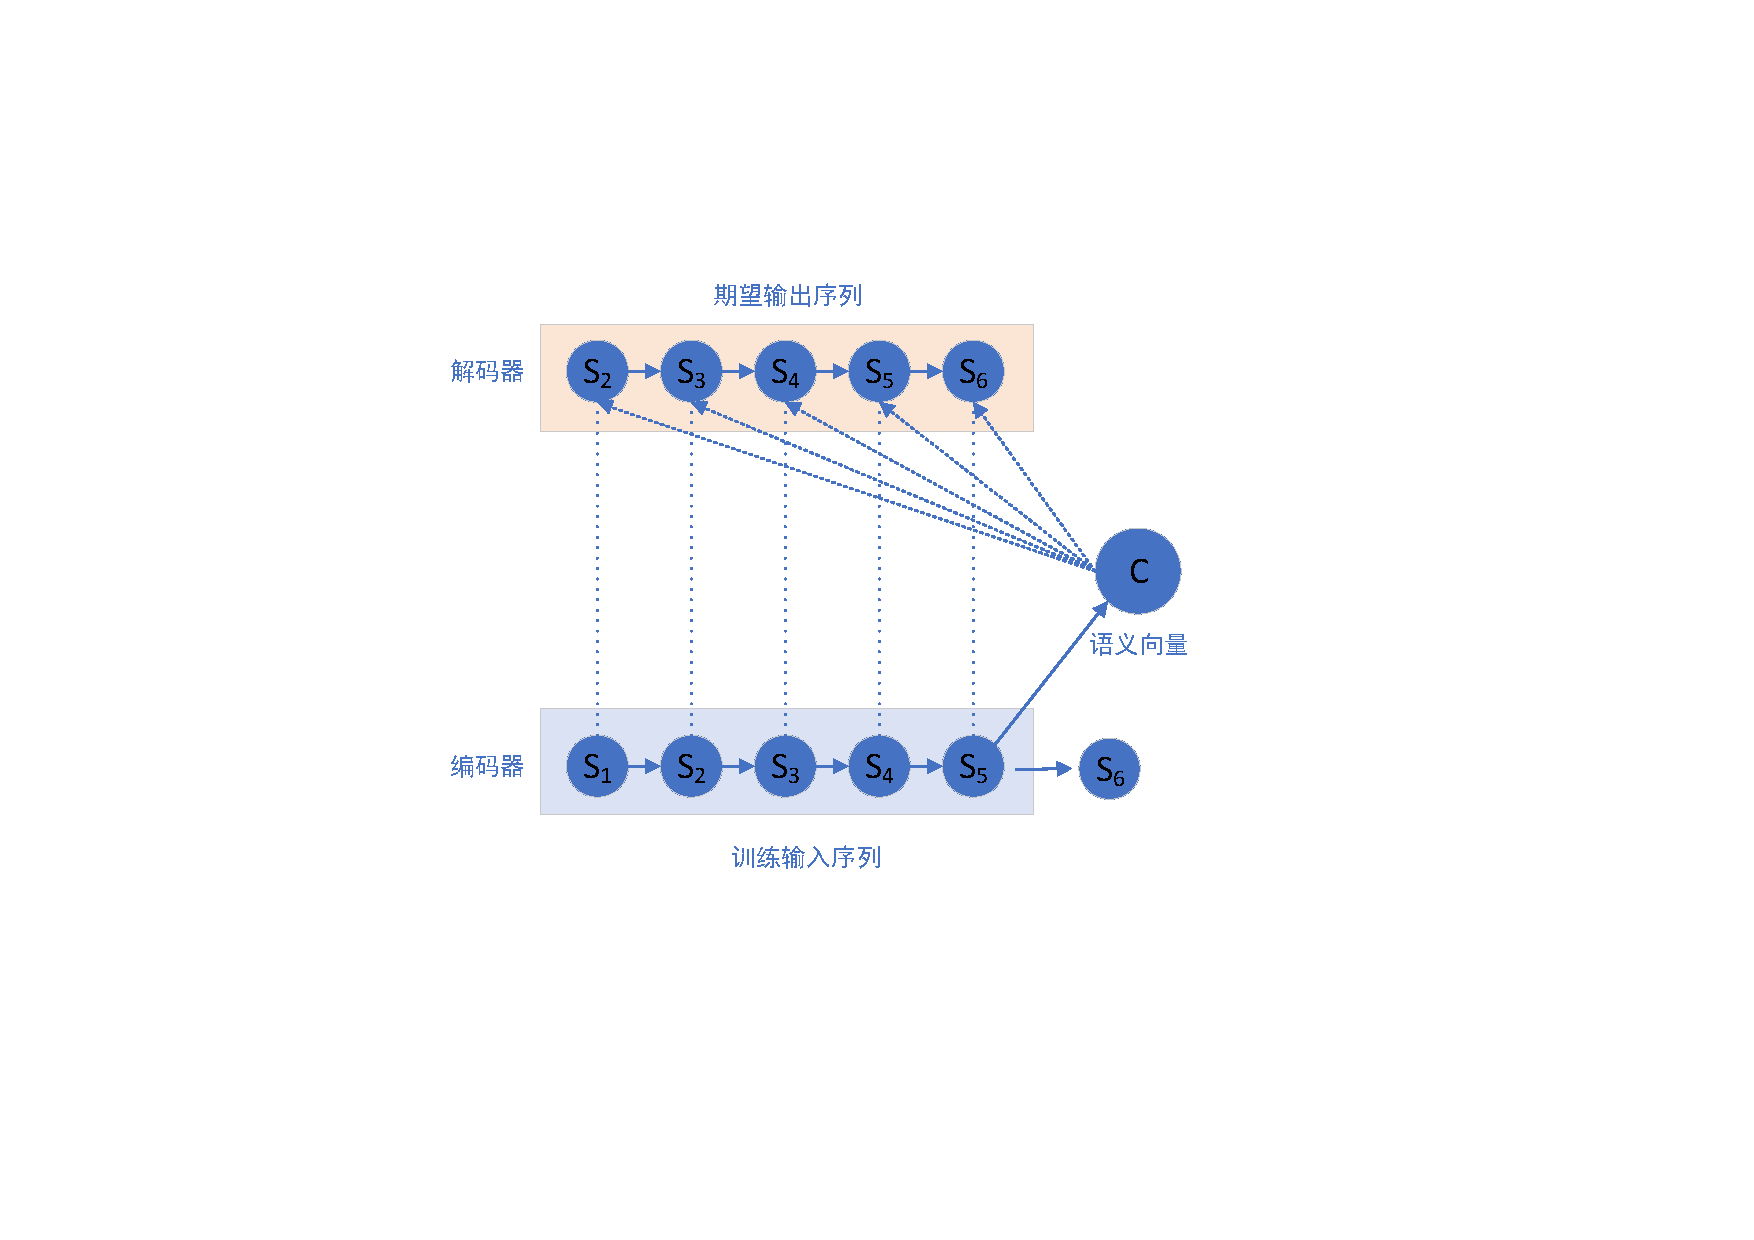
\includegraphics[height=6cm]{encoder-decoder.pdf} %,width=8cm
\caption{Encoder-Decoder框架结构示意图}
\label{encoder}
\end{figure}


输入节点$s_{1}$,其对应的期望后继节点应为$s_{2}$,输入节点$s_{5}$,其期望的后继节点应为$s_{6}$。由于循环神经网络自身结构导致的难以并行训练问题,Encoder和Decoder的特征提取下我们准备选用自注意模型,下面对自注意模型的构建方式进行了介绍。

\section{自注意力模块}

自注意力方法是一种特殊的注意力机制,已有在各种任务上的成功应用。与最简单的注意力方法通过对%
整个语境学习得到有限的知识表示不同,自注意力方法即使面对相隔距离较远的两个元素,其依然能%
保存上下文中的序列信息并且捕获这两个元素在序列上的关系。因此我们这里使用自注意力方法来捕获%
用户历史行为中的序列特征。

构建自注意力模块的基本单元由\textit{缩放点乘注意力Scaled Dot-product Attention}构成,%
一个自注意力模块的输入由\textit{查询(query)},\textit{键(key)}和\textit{值(value)}%
三部分组成。自注意力模块的输出是模块中\textit{值(value)}的加权和得来,而这里的权重矩阵则有%
\textit{查询(query)}和其对应的\textit{键(key)}决定。

我们用$Q$表示\textit{查询(query)}向量,用$K$表示\textit{键(key)}向量,用$V$表示%
\textit{值(value)}向量,向量中的每一行代表一个物品。首先,我们通过使用共享参数的非线性%
变换将\textit{查询}和\textit{键}投影到同一空间:
\begin{align} 
	Q^{\prime} &=\operatorname{ReLU}(W_{Q}\widehat{\mathbf{E}}) \\ 
	K^{\prime} &=\operatorname{ReLU}(W_{K}\widehat{\mathbf{E}})
\end{align}

其中$W_{Q}$,$W_{K}$分别是\textit{查询}和\textit{键}向量的权重矩阵,%
得到$Q^{\prime}$和$K^{\prime}$之后我们就可以通过如下形式得到\textit{值(value)}%
的权重矩阵:
\begin{align} 
	V^{\prime}=\operatorname{softmax}(\frac{Q^{\prime} {K^{\prime}}^{T}}{\sqrt{d}})
\end{align}
其中$\sqrt{d}$为缩放因子,为了避免点乘之后出现过大的值导致softmax的输出被推到梯度消失的%
位置,因此加上缩放因子来优化矩阵点乘。于是Self-Attention模块的输出就可以计算出来了:
\begin{align} 
	\mathbf{S}=\mathrm{SA}(\widehat{\mathbf{E}})=\text { Attention }(W_{Q}\widehat{\mathbf{E}}, W_{K}\widehat{\mathbf{E}}, W_{V}\widehat{\mathbf{E}}) = V^{\prime}\widehat{\mathbf{E}}
\end{align}

\textbf{多头注意力机制Multi-Head Attention}
{}
与其只让单个Self-Attention模块来学习$d$维的\textit{查询(query)},\textit{键(key)}和\textit{值(value)},可以通过集成学习的方法,让多个Self-Attention模块分别学习不同位置子空间的表达,由于随机初始化的不同,每个Self-Attention模块的关注点将会有所差异,所以每个Self-Attention模块可以分别学习到三个不同的$d_{k}$维的\textit{查询(query)}、$d_{k}$维的\textit{键(key)}和$d_{v}$维的\textit{值(value)}向量。每个Self-Attention模块有了\textit{查询(query)}、\textit{键(key)}和\textit{值(value)}之后,就能得到$d_{v}$维的输出。而Multi-Head Attention是多个Scaled Dot-product Attention的并行叠加,因此Multi-Head Attention的计算复杂度与Scaled Dot-product Attention相当,但是却获得了更好的泛化性能。因此这部分Multi-Head Attention的计算方式如下:
\begin{align} 
	\text { MultiHead }(\widehat{\mathbf{E}}) =\text { Concat }[\mathrm{SA}_{1}(\widehat{\mathbf{E}}), \ldots, \mathrm{SA}_{h}(\widehat{\mathbf{E}})] W^{O}
\end{align}
其中$h$表示我们将$h$个Self-Attention模块并联堆叠在一起得到Multi-Head Attention模块。

\begin{figure}[!htb]
   \begin{minipage}{0.48\textwidth}
     \centering
     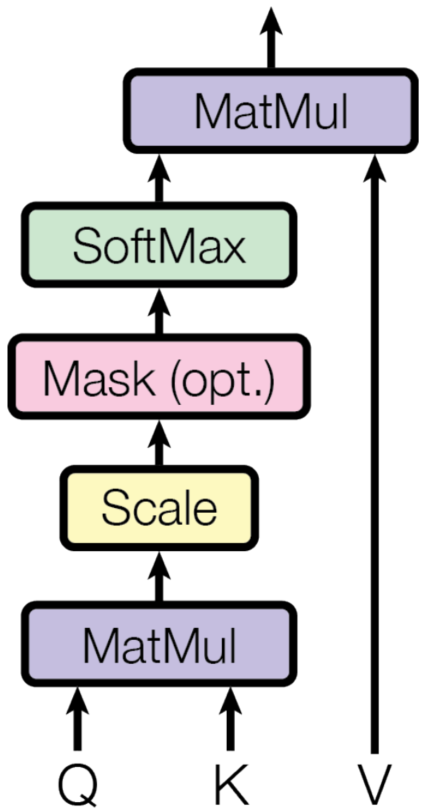
\includegraphics[height=6cm]{Scaled_Dot-Product_Attention.png} % ,width=\linewidth
     \caption{Scaled Dot-Product Attention缩放点乘注意力结构图}
     \label{Fig:Scaled_Dot-Product_Attention}
   \end{minipage}\hfill
   \begin {minipage}{0.48\textwidth}
     \centering
     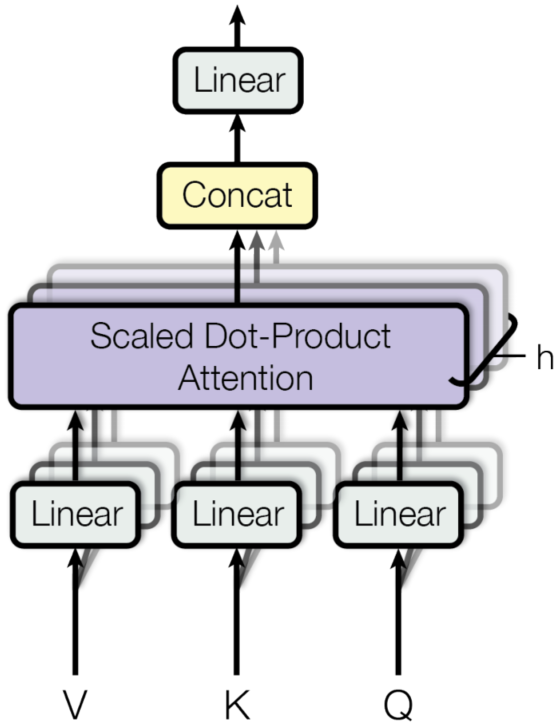
\includegraphics[height=6cm]{Multi-Head_Attention.png} % ,width=\linewidth
     \caption{Multi-Head Attention多头注意力模块结构图}
     \label{Fig:Multi-Head_Attention}
   \end{minipage}
   % \caption{BiLSTM4Rec training}
   % \label{fig:coffee}
\end{figure}

\textbf{结构中逐项的feed-forward网络作用}

考虑到Self-Attention模块在学习物品嵌入向量的过程中仍然是一个广义线性模型,为了增强整个Transformer模型的非线性拟合能力,Multi-Head Attention子层后面跟了一个前馈神经网络FFN层,为了保证模型计算的效率,它仅由两个线性变换组成,中间嵌入一个Relu激活函数来提升非线性表达能力,因此这一部分的形式如下:
\begin{align}
	\mathbf{F}_{i}=\mathrm{FFN}\left(\mathbf{S}_{i}\right)=\operatorname{ReLU}\left(\mathbf{S}_{i} \mathbf{W}^{(1)}+\mathbf{b}^{(1)}\right) \mathbf{W}^{(2)}+\mathbf{b}^{(2)}
\end{align}
其中$\mathbf{S}_{i}$表示嵌入层经过第$i$个Self-Attention模块计算后的输出

\textbf{Residual Connections残差连接}

在序列建模的问题当中,用户最后一个点击浏览的物品通常会与下一个物品的联系较大,所以最后一个物品的特征权重应该会更大。由于Self-Attention模块在处理最后一个物品的嵌入向量的时候会将其与之前所有的其他物品嵌入向量做交互,因此最后一个物品的特征并没有特别关注。为了提升对这种浅层特征的提取能力,可以为模型增加残差连接操作,其主要思想是如果浅层特征对于目标学习有效的话,就直接将低层网络学习的浅层特征直接传递给输出层,而不用再经过深层网络提取复杂特征,残差连接的做法就是将浅层网络的输出建立旁路与输出层相连,跳过了部分中间复杂计算。

\begin{figure}
\centering
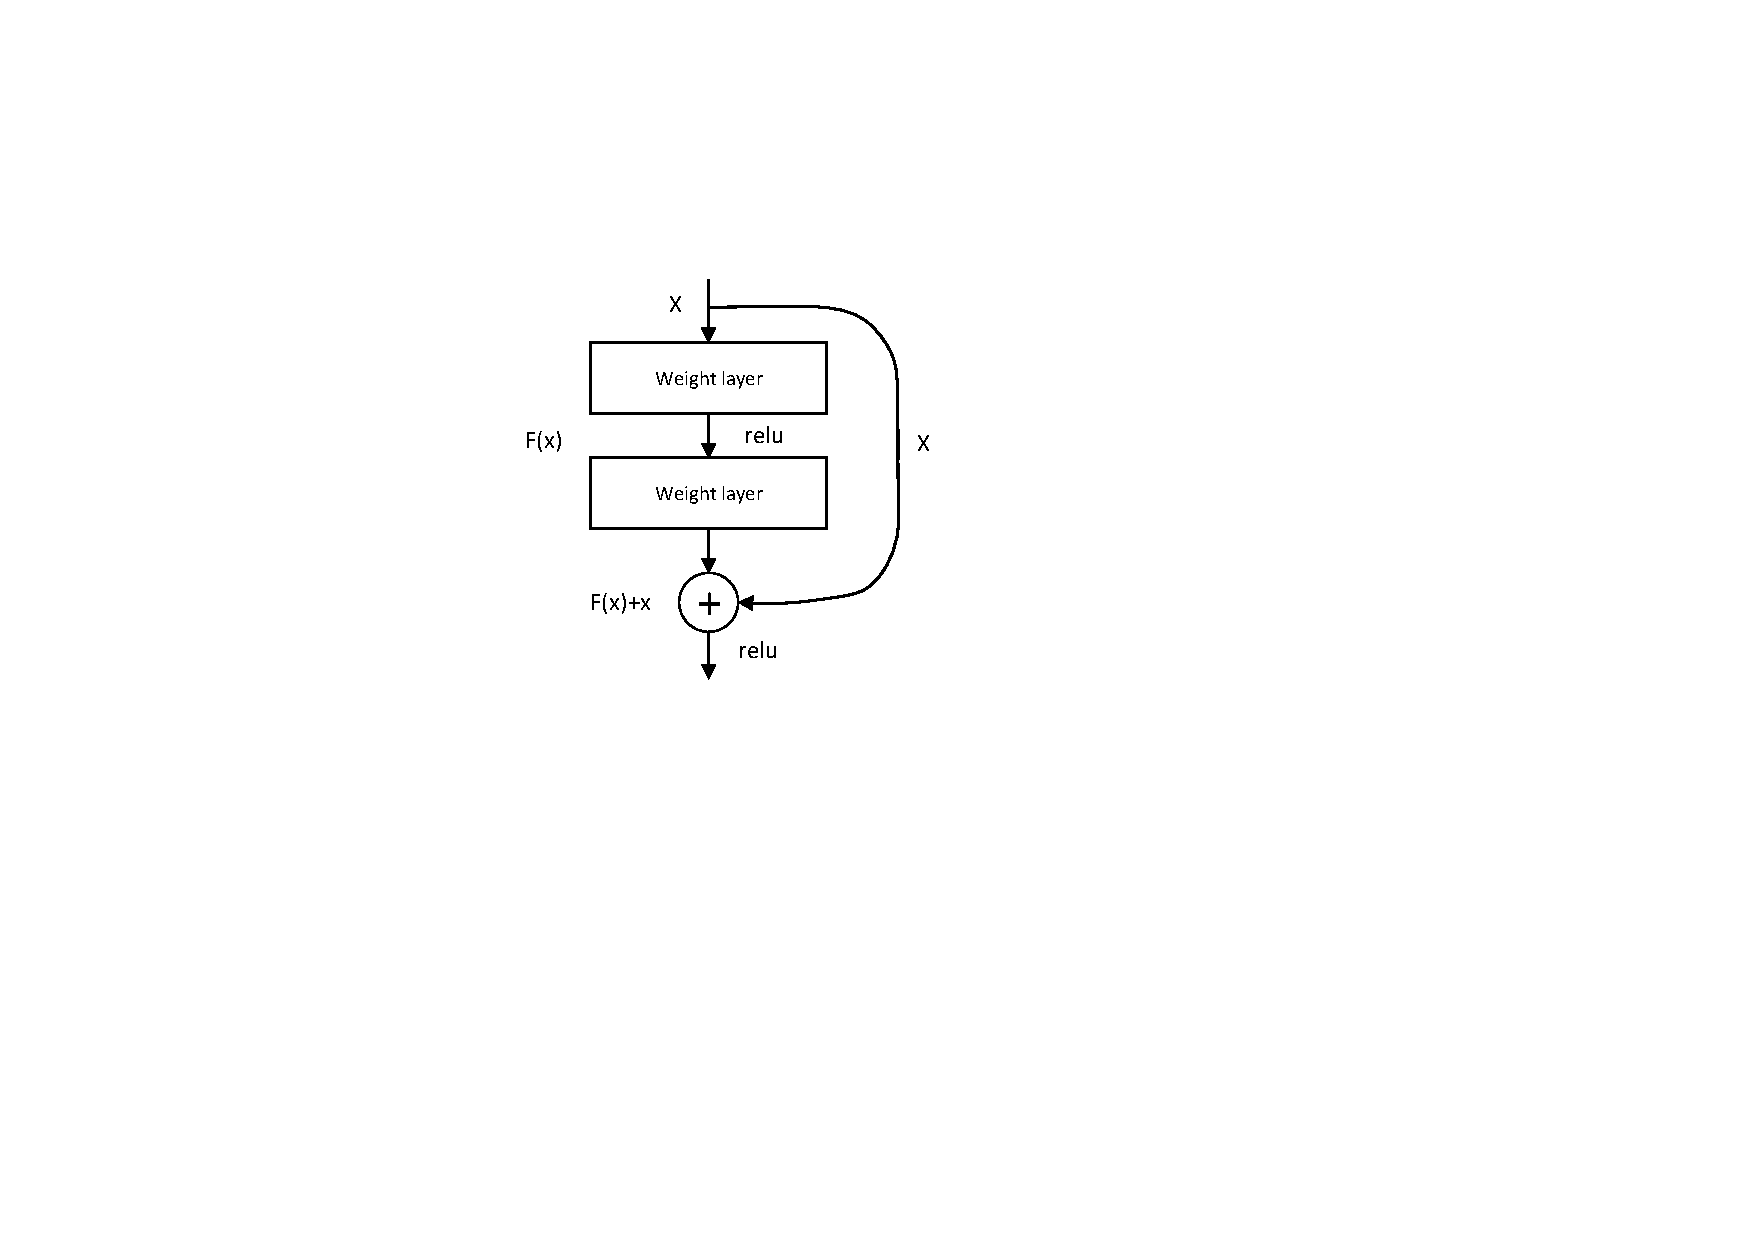
\includegraphics[height=6cm]{residual.pdf}
\caption{残差连接结构图}
\label{residual}
\end{figure}

\textbf{层次归一化Layer normalization}

为了使得模型训练的时候更加容易收敛,减少训练时间,在深度神经网络的模型中加入归一化操作是一个比较常见的做法。在训练卷积神经网络时候,常见的操作是加入批量归一化(Batch Normalization)\upcite{Ioffe:2015:BNA:3045118.3045167},批量归一化通过计算均值和方差将一个批量的输入数据装换到$[0,1]$之间,加速梯度下降,但其高度依赖批量的大小,同时也不适用于输入序列长度不固定的循环神经网络等模型。层次归一化(Layer Normalization)\upcite{ba2016layer}则不是在样本层面,而是将该层神经元的输入通过计算均值和方差转换到在$[0,1]$之间,这样的操作是跨特征计算的,与其他样本无关,因此可以使用任意大小的批量大小。
\begin{align}
	LN(x_i)=\alpha\times\frac{x_i-u_B}{\sqrt{\sigma_B^2+\epsilon}}+\beta
\end{align}
\textbf{Dropout}

使用神经网络时,随着模型变得更大和更深,也带了过拟合的潜在风险,对于神经网络来说,除了在损失函数处加上L1和L2正则项之外,在模型的结构当中加入Dropout也是防止过拟合的常见操作之一,为了防止我们的模型过拟合、同时为了让训练更稳定,减少部分模型参数加速训练过程,在Self-Attention模块的输出之后加上Dropout操作:
\begin{align}
	\hat{y}=x+\text { Dropout }(\text {SA}(\text { LN }(x)))
\end{align}
\textbf{模型训练}
最终模型根据输出序列是否为用户实际点击行为经过$Sigmoid(\cdot )$函数映射到$[0,1]$之间的概率,因此模型的优化目标为最小化如下的交叉熵损失函数:
\begin{align}
-\sum_{{u} \in \mathbb{U}} \sum_{t \in[1,2, \ldots, n]}\left[\log (\hat{y})+\sum_{\hat{s}_{u}^{t}\neq s_{u}^{t}} \log (1-\hat{y})\right]
\end{align}




\section{复杂度分析}

模型的时间复杂度只要由Self-Attention模块主导,Self-Attention的时间复杂度为$O(n^{2} d)$,其中$n$为序列的长度,$d$为嵌入层维度,而Multi-Head Attention由多个Self-Attention并行叠加,假设有$h$个Self-Attention,则Multi-Head Attention的时间复杂度仍为$O(n^{2} d)$,


% \subsection{算法描述}


\subsection{算法实现}
\begin{algorithm}[H]
	\caption{基于自注意力机制的序列感知推荐算法}
	\label{alg:self-attention}
		\begin{algorithmic}[1]
			\REQUIRE 用户序列数据:$S$;最大序列长度:$maxLen$; 最大字数:$maxNum$
			\ENSURE 推荐结果列表:$Items$
			\STATE $sequences \leftarrow S$, 其中$sequences=\{sen_{1}, sen_{2}...sen_{n}\}$ 
			\FOR {$sequence$ in $input\_sequences$}
			    \STATE $embedding\_sequence()$
			    \STATE $pos\_embedding\_sequence()$
				    \FOR {$Self\_Attention$ in $Multi\_Head\_Attention$}
					    \STATE do $Self\_Attention$()
					    \STATE do $Layer\_Normalize$()
					    \STATE do $FeedForward$()
					    \STATE $input\_sequence$ = $sequence$*Mask
					\ENDFOR
			\ENDFOR
			\FOR {$sequence$ in $output\_sequences$}
			    \STATE $embedding\_sequence()$
			    \STATE $pos\_embedding\_sequence()$
				    \FOR {$Self\_Attention$ in $Multi\_Head\_Attention$}
					    \STATE do $Self\_Attention$()
					    \STATE do $Layer\_Normalize$()
					    \STATE do $FeedForward$()
					    \STATE $output\_sequence$ = $sequence$*Mask
					\ENDFOR
			\ENDFOR
			\STATE $sequence$ = $output_sequence$ + $input_sequence$
			\STATE do $Layer\_Normalize$()
			\FOR {$Self\_Attention$ in $Multi\_Head\_Attention$}
			    \STATE do $Self\_Attention$($sequence$)
			    \STATE do $Layer\_Normalize$($sequence$)
			    \STATE do $FeedForward$($sequence$)
			\ENDFOR
			\STATE $output$ = $Sigmoid(sequence)$
			\STATE $NextItem = Max(output) $
			\RETURN $NextItem$
		\end{algorithmic}
\end{algorithm}


\section{本章小结}

本章节主要针对基于(双向)循环神经网络的序列感知推荐算法难以并行训练的缺点,采用自注意力机制,更进一步提升序列感知推荐算法的性能
介绍本文提出的另外一个基于自注意力机制的序列感知推荐算法,其虽然抛弃了循环神经网络的递归结构,但引入位置信息编码的方式仍然能够捕获到序列位置的变化情况,没有了递归的结构依赖,也使得该模型的训练更容易并行化实现,在不损失推荐结果排序准确性的情况下还能获得较高的性能。

